\documentclass[11pt]{article}
% !TEX root = LaTeX.tex

%%%%%%%%%%%%%%%%%%%
% Page Layout
%%%%%%%%%%%%%%%%%%%

\setlength{\paperwidth}{8.5in} \setlength{\paperheight}{11in}
\setlength{\marginparwidth}{0in} \setlength{\marginparsep}{0in}
\setlength{\oddsidemargin}{0in} \setlength{\evensidemargin}{0in}
\setlength{\textwidth}{6.5in} \setlength{\topmargin}{-0.5in}
\setlength{\textheight}{9in}

%%%%%%%%%%%%%%%%%%%%%%%%%%%%%%%%%%%
% Include Packages and Style Files
%%%%%%%%%%%%%%%%%%%%%%%%%%%%%%%%%%%

\usepackage[english]{babel}
\usepackage{amsmath,amssymb,amsthm}
\usepackage{enumerate}
\usepackage{xcolor}
\usepackage[useregional]{datetime2}
\usepackage[pdftex]{graphicx,color}
\usepackage{graphicx}
\graphicspath{ {M5600/} }

%%%%%%%%%%%%%%%%%%%%%%%%%%%%%%
% Define theorem environments
%%%%%%%%%%%%%%%%%%%%%%%%%%%%%%

\newtheorem{theorem}{Theorem}[section]
\newtheorem{proposition}[theorem]{Proposition}
\newtheorem{lemma}[theorem]{Lemma}
\newtheorem{corollary}[theorem]{Corollary}
\newtheorem{claim}[theorem]{Claim}
\newtheorem{question}[theorem]{Question}
\newtheorem{conjecture}[theorem]{Conjecture}

\theoremstyle{definition}
\newtheorem{definition}[theorem]{Definition}
\newtheorem{example}[theorem]{Example}
\newtheorem*{remark}{Remark}

%%%%%%%%%%%%%%%%%%%%%%
% Define new commands
%%%%%%%%%%%%%%%%%%%%%%

\newcommand{\R}{\mathbb{R}}


\newcommand{\E}{\mathbb{E}}
\renewcommand{\P}{\mathbb{P}}
\newcommand{\Var}{\operatorname{Var}}
\newcommand{\1}[1]{\mathbf{1} \left \{ #1 \right \}}
\newcommand{\Range}{\operatorname{Range}}

%%%%%%%%%%%%%%%%%%%%%%

\begin{document}

\title{Numerical Analysis Project \\ MATH 5600 \\ Homework 1}
\date{Due: February 10, 2021}
\author{Authors: \\ Dane Gollero \\ Ike Griss Salas \\ Magon Bowling}

\maketitle

\section*{\textbf{Models of the Earth with Respect to Coordinate Systems}}
In our work through the term project, we utilize two coordinate systems: Geographical and Cartesian.  Geographical coordinates are used to identify a location on the Earth in terms of Longitude and Latitude.  In relationship with Cartesian coordinates, Geographic coordinates rotate around the z-axis with respect to time.  At time = 0, the x-axis intersects the globe at the Equator and Prime Meridian.  The y-axis therefore perpendicular to the xz-plane.
\[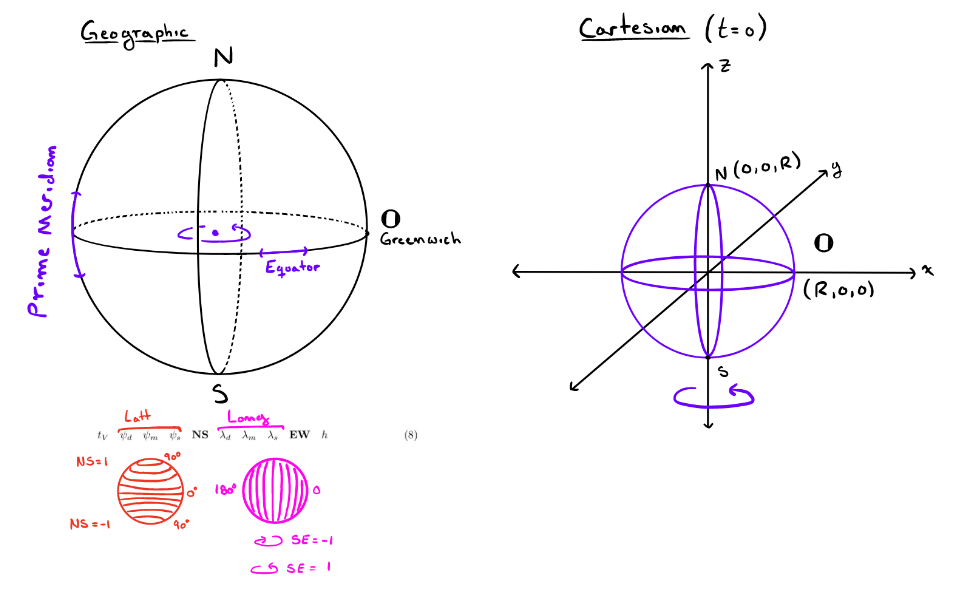
\includegraphics[width=15cm, height=9cm]{M5600/Images/M5600_EarthModels.PNG}\]

\begin{itemize}
\item[{\textbf{Exercise 1:}}] Find a formula that describes the trajectory of the point \textbf{O} in Cartesian coordinates as a function of time.

From Physics, we know that distance is equal to the rate of an object multiplied by the time traveled.  We can apply this to trajectory with the equation $\theta = \omega \cdot t$, where $\omega$ is angular velocity.  Angular velocity is the distance around the globe divided by one sidereal day.  Thus we obtain the angle $\theta = \frac{2\pi}{s} \cdot t$.  The formula that describes the trajectory of the point \textbf{O} as a function of time in Cartesian coordinates is: \\
\[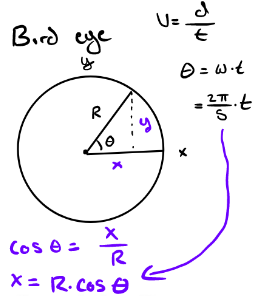
\includegraphics[width=0.15\textwidth]{M5600/Images/M5600_theta_2pi_s.PNG}\]
\[\textbf{O}_{car}(t) =
\begin{bmatrix}
R \cos{\big(\frac{2pi}{s}\big) \cdot t} \\
R \sin{\big(\frac{2pi}{s}\big) \cdot t} \\
0
\end{bmatrix}
\]
\\
\item[{\textbf{Exercise 2:}}] Write a program that converts angles from degrees, minutes, and seconds to radians, and vice versa.
\[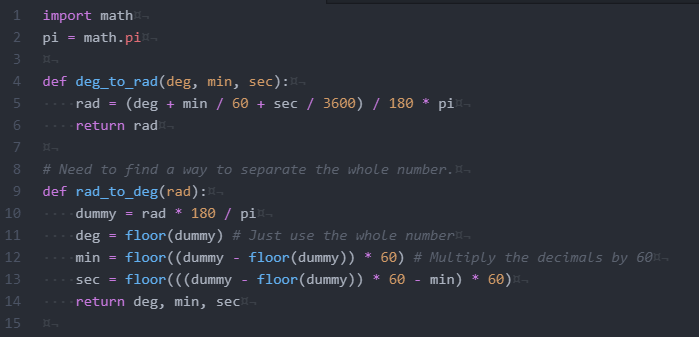
\includegraphics{Images/M5600_2_Code.PNG}\]
\\
\item[{\textbf{Exercise 3:}}] Find a formula that converts position as given in (8) at time $t = 0$ into Cartesian coordinates.
It is important to note the parameters for the following variables: \\
\(t_V = 0\) \(\psi_d, \psi_m, \psi_s \in \big[0, \frac{pi}{2}\big]\)

\end{itemize}

\end{document}
